\section{Shape Index and Query-Shape Containment}

\begin{figure}[h!]
    \centering
    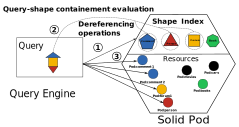
\includegraphics[width=0.7\textwidth]{figure/shape_containement}
    \caption{First, the shape index is dereferenced, 
    then the \emph{query-shape containment} operations are performed in the query engine and lastly, only the relevant resources are dereferenced.}
    \label{fig:shape_index}
\end{figure}

\sepfootnotecontent{fn:shapetrees}{
    \href{https://shapetrees.org/TR/specification/}{https://shapetrees.org/TR/specification/}
}

\sepfootnotecontent{fn:solidPrivacy}{
In this work, we do not take into consideration confidentiality restrictions.
}

\sepfootnotecontent{fn:litShapeComparaison}{
There exist comparisons between the shape and class definition approaches in the context of data validation~\cite{demeester_swj_2021} but it is left to be determined if their frame of comparison is compatible with our current problem
and foreseen opportunities.
}
\sepfootnotecontent{fn:domain}{
From a perspective where the domain is composed of URLs leading to linked data documents and the codomain is composed of the documents with their RDF content.
}

The RDF specification does not enforce schemas on data.
However, the data published often adhere to an implicit schema due to the nature of its modeled object and the formulation of RDF~\cite{Neumann2011CharacteristicSA}.
From those observations, implicit schemas have been used with success for query optimization~\cite{Neumann2011CharacteristicSA, Meimaris2018HierarchicalCS}.
We propose to adapt those methods for LTQP by using explicit data schemas provided by the data provider in our source selection process.

Our method introduces the concept of a \emph{shape index} to reduce query execution time by minimizing unnecessary dereferencing of RDF documents within web subdomains (sets of URLs or URL patterns)~\sepfootnote{fn:domain}.
We define a shape index as a set of mappings between RDF data shapes and sets of resources.
This mapping concept shares similarities with shape mapping~\cite{Gayo2018} and target declarations~\cite{Gayo2018Shacl}.
However, instead of mapping shapes to RDF subgraphs, the shape index maps shapes to sets of documents.
The shape index also shares commonalities with \href{https://shapetrees.org/}{shape trees}~\sepfootnote{fn:shapetrees}, however, it is designed to be a simpler formulation focused on query optimization.
The shape index has a range of applications defined in a domain and a flag indicating if the index is \emph{complete}.
A shape index is complete when every resource in the domain is associated with a shape within the shape index.
In a shape index when a shape is mapped to a set of RDF resources then the shape \emph{must} validate those resources.
Furthermore, every set of triples respecting the shape in the domain \emph{must} be located inside one resource of the set.

In order to determine before the traversal of a whole subdomain which resources are useful and which can be pruned, the query engine solves a \emph{query-shape containment} problem over the shape of the index analogous to the classic query containment problem~\cite{afariQCE, Spasi2023, Chekol2018}.
The query containment problem consists of determining independent of the data source if the results of a query will be a subset of the results of another query.
We propose to express RDF data shapes into select SPARQL queries ($Q_{s}$)~\cite{delva2023, spapeExpressionConvert, labragayo2017validating, Corman2019} and apply similar resolution methods to query containment problems.
Due to the explicit domain definition of the index, this approach is adaptative, 
thus, the query engine can start its processing with permissive reachability criteria
such as $c_{all}$~\cite{Hartig2012} or the Solid state-of-the-art reachability criteria~\cite{Taelman2023}
and not suffer from the associated longer execution time during the traversal of environments containing a shape index.
The source selection process is schematized for a single (sub)domain in Figure~\ref{fig:shape_index}.
The process starts with the discovery of the shape index in the current (sub)domain.
In the case of Solid, the index can be at the root of the pod to be easily discoverable~\sepfootnote{fn:solidPrivacy}.
After the dereferencing of the index, the analysis is started inside the query engine.
The analysis consists of interpreting the binding results (homomorphism and "partial" homomorphism) of the \emph{query-shape containment} problem.
The algorithm divides the query from the user into multiple star patterns with their dependent star pattern ($Q_{star}$).
After the division of the query, the queries are pushdown~\cite{Stuckenschmidt2004, Yang2021FlexPushdownDBHP} to the level of source selection to evaluate if the $Q_{star}$ are contained inside the $Q_s$ of the shape index.
If all the $Q_{star}$ are contained in a $Q_{s}$ or have no binding with any $Q_{s}$
the reachability criterion is adapted to ignore all the resources not linked to a $Q_{s}$ even if the shape index is \emph{incomplete}.
If the shape index is \emph{complete} and not all the $Q_{star}$ are contained in a $Q_{s}$ the reachability criterion can be adapted
to visit every resource in relation to a $Q_{s}$ with a partial binding with a $Q_{star}$.
In a similar case with an \emph{incomplete} shape index, the query engine can only use the shape index for data discovery.
This case is similar to the usage of the type index but with a more reaching ability to match a query with the index because shapes in their definition describe the properties (RDF predicates) of the entities whereas the type index only provides the classes IRIs.
It is possible to dereference the class IRIs to get information about the properties (if available), however, it is not the current practice \cite{Taelman2023}.
A comparison of the RDF data shapes and RDF class approach due to their potential similarities is delegated to future works~\sepfootnote{fn:litShapeComparaison}.

We conclude this section with a concrete example.
Let's assume that a user wants to request every ID and content of the comments in the networks with the forums where they have been posted and the capital of the countries where the forum has been created.
Conceptually, we \emph{can} imagine a situation with four star pattern query entities, the comments $ Q_{comments}$, the forum $Q_{forums}$, and the countries $Q_{countries}$.
The user's query is formed by the join of those star patterns, with consideration of the dependencies between them induced by the definition of variables with the same name $Q = Q_{comments} \bowtie Q_{forums} \bowtie Q_{countries}$. 
When traversing a part of the networks the engine cannot know what is inside the documents hence it is preferable for it to dereference all the reachable ones given a defined reachability criteria.
The presence of a shape index can make the state of affairs different.
If a domain only contains books data as advertised by a shape index via a shape mapping, all its documents can be skipped entirely 
whereas if a domain has comments and pasta recipes data the query engine can know it can safely limit its dereferencing operations to the set of documents related to comments without affecting results completeness given the index is complete.
The engine can do as such because at least one star pattern is contained in the comment shape and none in the pasta shape.
If we have a domain that is incomplete but advertises comments, forums, and countries at least then the documents associated with the rest of the domain can be ignored.
Thus, we can consider that the traversal proceeds domain by domain requesting document sets known a priori to be not in contradiction with the star pattern queries until no new documents are reachable or a limit clause is satisfied.
